\documentclass{article}

\usepackage[margin=1in]{geometry}
\usepackage{graphicx} % Allow image/pdf includes
\usepackage{extramarks} % Extra header marks (continued on next page)
\usepackage{amsmath} % Math enhancements
\usepackage{amsthm} % Theorem typesetting
\usepackage{amssymb} % Extended symbol collection
\usepackage{tikz} % Graphical element creation
\usetikzlibrary{automata,positioning}
\usepackage{algpseudocode} % Algorithm layout
\usepackage{enumitem} % Enumerate (lists)
\usepackage{ragged2e} % Alternative alignment
\usepackage{gensymb} % Generic symbols (degree, etc)
\usepackage{empheq} % Allow \boxed around \begin{empheq}
\usepackage{color,soul} % Highlighting
\usepackage{booktabs} % Enhanced table creation
\usepackage{multirow} % Table multi row
\usepackage{mathtools} % Math enhancements
\usepackage{bm} % Bold math
\usepackage[mathscr]{euscript} % Script variables
\usepackage{cancel} % Cancel through text
\usepackage{color,soul} % Highlighting
\usepackage{mathtools}
\usepackage{multirow}
\usepackage{mathrsfs}
\usepackage{physics}
\usepackage{gensymb}
\usepackage{siunitx}
\usepackage{subcaption}
\usepackage[]{algorithm2e}
\usepackage{float}
\usepackage[cache=false]{minted}
\renewcommand{\MintedPygmentize}{/Users/logan/miniconda/bin/pygmentize}
\usepackage[scaled]{beramono}
\usepackage[T1]{fontenc}

\setlength\parindent{0pt} % No indents
\setlength{\parskip}{1em} % Paragraph skip

\newcommand{\vx}{\mathbf{x}} % x vector
\newcommand{\vy}{\mathbf{y}} % x vector

\newcommand{\pageTitle}{MEEN 644 - Homework 4}
\newcommand{\pageAuthor}{Logan Harbour}

\begin{document}

\title{\LARGE \textbf{\pageTitle} \vspace{-0.3cm}}
\author{\large \pageAuthor}
\date{\vspace{-0.6cm} \large \today \vspace{-0.4cm}}

\maketitle

\section*{Problem statement}

Consider a thin copper square plate of dimensions 0.5 m $\times$ 0.5 m. The temperature of the west and south edges are maintained at 50 $^\circ$C and the north edge is maintained at 100 $^\circ$C. The east edge is insulated. Using finite volume method, write a program to predict the steady-state temperature solution.

\begin{enumerate}[label=(\alph*)]
	\item \textbf{(35 points)} Set the over relaxation factor $\alpha$ from 1.00 to 1.40 in steps of 0.05 to identify $\alpha_\text{opt}$. Plot the number of iterations required for convergence for each $\alpha$.
	\item \textbf{(15 points)} Solve the same problem using $21^2, 25^2, 31^2$, and $41^2$ CVs, respectively. Plot the temperature at the center of the plate (0.25 m, 0.25 m) vs CVs.
	\item \textbf{(10 points)} Plot the steady state temperature contour in the 2D domain with the $41^2$ CV solution.
\end{enumerate}

\section*{Preliminaries}

\subsection*{Two-dimensional heat conduction}

With two-dimensional heat conduction with constant material properties, insulation on the right and prescribed temperatures on all other sides, we have the PDE
\begin{equation}
	\begin{cases}
		k \pdv{^2T}{x^2} + k \pdv{^2T}{y^2} = 0\,,\\
		T(x, 0) = T_B\,,\\
		T(0, y) = T_L\,,\\
		T(0, L_y) = T_T\,,\\
		-k \pdv{T}{x} \Big|_{x = L_x} = 0\,,
	\end{cases}
\end{equation}
where
\begin{align*}
	T_B & \equiv 50~^\circ\text{C}\,, & T_L & \equiv 50~^\circ\text{C}\,, & T_T & \equiv 100~^\circ\text{C}\,.\\
	k & \equiv 386~\text{W/m}~^\circ\text{C}\,, & L_x & \equiv 0.5~\text{m}\,, & L_y & \equiv 0.5~\text{m}\,.\\
\end{align*}

\subsection*{Control volume equations}

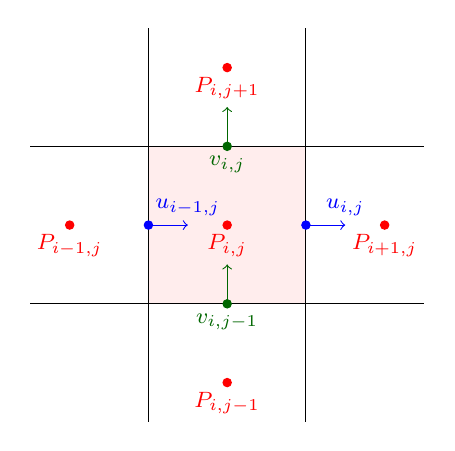
\begin{tikzpicture}[scale=1, style={font=\footnotesize}]
	\tikzset{dimen/.style={<->,>=latex,thin,every rectangle node/.style={fill=white,midway,font=\small}}}
	
	\filldraw[red!7] (0,0) -- (2,0) -- (2,2) -- (0, 2) -- cycle;
	\draw (-1.5, 0) -- (3.5, 0);
	\draw (-1.5, 2) -- (3.5, 2);
	\draw (0, -1.5) -- (0, 3.5);
	\draw (2, -1.5) -- (2, 3.5);
	
	\filldraw[red] (1, 1) circle (1.5pt);
	\filldraw[blue] (0, 1) circle (1.5pt);
	\filldraw[green!40!black] (1, 0) circle (1.5pt);
	\filldraw[blue] (2, 1) circle (1.5pt);
	\filldraw[green!40!black] (1, 2) circle (1.5pt);
	\filldraw[red] (-1, 1) circle (1.5pt);
	\filldraw[red] (3, 1) circle (1.5pt);
	\filldraw[red] (1, 3) circle (1.5pt);
	\filldraw[red] (1, -1) circle (1.5pt);
	
	\draw [->,blue] (0, 1) -- (0.5, 1);
	\draw [->,blue] (2, 1) -- (2.5, 1);
	\draw [->,green!40!black] (1, 0) -- (1,0.5);
	\draw [->,green!40!black] (1, 2) -- (1,2.5);
	
	\node[below, red] at (1, 1) {$P_{i, j}$};
	\node[below, red] at (3, 1) {$P_{i+1, j}$};
	\node[below, red] at (-1, 1) {$P_{i-1, j}$};
	\node[below, red] at (1, 3) {$P_{i, j+1}$};
	\node[below, red] at (1, -1) {$P_{i, j-1}$};
	
	\node[above,blue] at (0.5, 1) {$u_{i-1,j}$};
	\node[above,blue] at (2.5, 1) {$u_{i,j}$};
	\node[below,green!40!black] at (1, 0) {$v_{i,j-1}$};
	\node[below,green!40!black] at (1, 2) {$v_{i,j}$};
\end{tikzpicture}

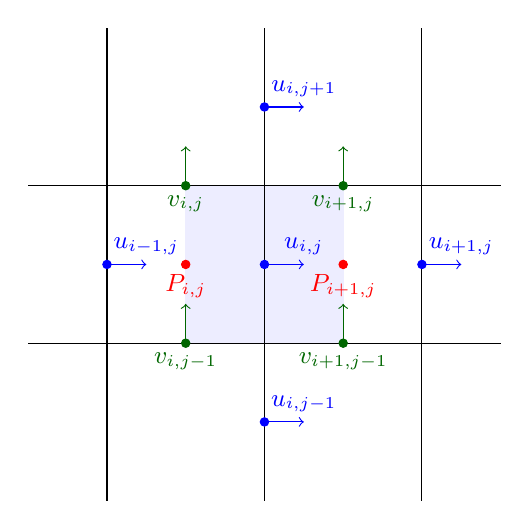
\begin{tikzpicture}[scale=1, style={font=\small}]
	\tikzset{dimen/.style={<->,>=latex,thin,every rectangle node/.style={fill=white,midway,font=\small}}}
	
	\filldraw[blue!7] (1,0) -- (3,0) -- (3,2) -- (1, 2) -- cycle;
	\draw (-1, 0) -- (5, 0);
	\draw (-1, 2) -- (5, 2);
	\draw (0, -2) -- (0, 4);
	\draw (2, -2) -- (2, 4);
	\draw (4, -2) -- (4, 4);
	
	\filldraw[red] (1, 1) circle (1.5pt);
	\filldraw[red] (3, 1) circle (1.5pt);
	\filldraw[green!40!black] (1, 2) circle (1.5pt);
	\filldraw[green!40!black] (1, 0) circle (1.5pt);
	\filldraw[green!40!black] (3, 0) circle (1.5pt);
	\filldraw[green!40!black] (3, 2) circle (1.5pt);
	\filldraw[blue] (2, 1) circle (1.5pt);
	\filldraw[blue] (4, 1) circle (1.5pt);
	\filldraw[blue] (0, 1) circle (1.5pt);
	\filldraw[blue] (2, 3) circle (1.5pt);
	\filldraw[blue] (2, -1) circle (1.5pt);
	
	\draw [->,blue] (0, 1) -- (0.5, 1);
	\draw [->,blue] (2, 1) -- (2.5, 1);
	\draw [->,blue] (4, 1) -- (4.5, 1);
	\draw [->,blue] (2, 3) -- (2.5, 3);
	\draw [->,blue] (2, -1) -- (2.5, -1);
	\draw [->,green!40!black] (1, 0) -- (1,0.5);
	\draw [->,green!40!black] (1, 2) -- (1,2.5);
	\draw [->,green!40!black] (3, 0) -- (3,0.5);
	\draw [->,green!40!black] (3, 2) -- (3,2.5);
	
	\node[below, red] at (1, 1) {$P_{i, j}$};
	\node[below, red] at (3, 1) {$P_{i+1, j}$};
	
	\node[above,blue] at (0.5, 1) {$u_{i-1,j}$};
	\node[above,blue] at (2.5, 1) {$u_{i,j}$};
	\node[above,blue] at (4.5, 1) {$u_{i+1,j}$};
	\node[above,blue] at (2.5, 3) {$u_{i,j+1}$};
	\node[above,blue] at (2.5, -1) {$u_{i,j-1}$};
	\node[below,green!40!black] at (1, 0) {$v_{i,j-1}$};
	\node[below,green!40!black] at (1, 2) {$v_{i,j}$};
	\node[below,green!40!black] at (3, 0) {$v_{i+1,j-1}$};
	\node[below,green!40!black] at (3, 2) {$v_{i+1,j}$};
\end{tikzpicture}

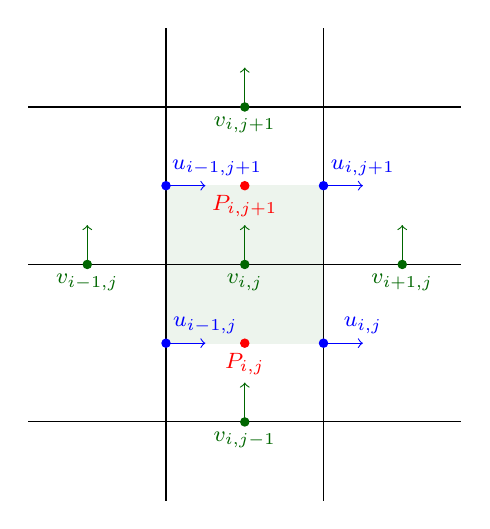
\begin{tikzpicture}[scale=1, style={font=\footnotesize}]
	\tikzset{dimen/.style={<->,>=latex,thin,every rectangle node/.style={fill=white,midway,font=\small}}}
	
	\filldraw[green!40!black!7] (0,1) -- (2,1) -- (2,3) -- (0, 3) -- cycle;
	\draw (-1.75, 0) -- (3.75, 0);
	\draw (-1.75, 2) -- (3.75, 2);
	\draw (-1.75, 4) -- (3.75, 4);
	\draw (0, -1) -- (0, 5);
	\draw (2, -1) -- (2, 5);
	
	\filldraw[red] (1, 1) circle (1.5pt);
	\filldraw[red] (1, 3) circle (1.5pt);
	\filldraw[blue] (0, 1) circle (1.5pt);
	\filldraw[blue] (2, 1) circle (1.5pt);
	\filldraw[blue] (0, 3) circle (1.5pt);
	\filldraw[blue] (2, 3) circle (1.5pt);
	\filldraw[green!40!black] (1, 0) circle (1.5pt);
	\filldraw[green!40!black] (1, 2) circle (1.5pt);
	\filldraw[green!40!black] (1, 4) circle (1.5pt);
	\filldraw[green!40!black] (-1, 2) circle (1.5pt);
	\filldraw[green!40!black] (3, 2) circle (1.5pt);
	
	\draw [->,blue] (0, 1) -- (0.5, 1);
	\draw [->,blue] (2, 1) -- (2.5, 1);
	\draw [->,blue] (0, 3) -- (0.5, 3);
	\draw [->,blue] (2, 3) -- (2.5, 3);
	\draw [->,green!40!black] (1, 0) -- (1,0.5);
	\draw [->,green!40!black] (1, 2) -- (1,2.5);
	\draw [->,green!40!black] (1, 4) -- (1, 4.5);
	\draw [->,green!40!black] (-1, 2) -- (-1, 2.5);
	\draw [->,green!40!black] (3, 2) -- (3, 2.5);
	
	\node[below, red] at (1, 1) {$P_{i, j}$};
	\node[below, red] at (1, 3) {$P_{i, j+1}$};
	\node[above,blue] at (0.5, 1) {$u_{i-1,j}$};
	\node[above,blue] at (2.5, 1) {$u_{i,j}$};
	\node[above,blue] at (0.65, 3) {$u_{i-1,j+1}$};
	\node[above,blue] at (2.5, 3) {$u_{i,j+1}$};
	\node[below,green!40!black] at (1, 2) {$v_{i,j}$};
	\node[below,green!40!black] at (1, 0) {$v_{i,j-1}$};
	\node[below,green!40!black] at (1, 4) {$v_{i,j+1}$};
	\node[below,green!40!black] at (-1, 2) {$v_{i-1,j}$};
	\node[below,green!40!black] at (3, 2) {$v_{i+1,j}$};
\end{tikzpicture}

\subsection*{Velocity update}

Define the Pechlet number on each boundary of a control volume $c_{i,j}$ as
\begin{equation}
	P^{c_{i,j}}_b = \frac{F^{c_{i,j}}_b}{D^{c_{i,j}}_b} \,, \quad \text{where} \quad b = [n, e, s, w] \quad \text{and} \quad c = [u, v]\,,
\end{equation}
where
\begin{subequations}
	\begin{align}
		D^{c_{i,j}}_n & = \frac{\Delta x \mu}{\Delta y}\,,\\
		D^{c_{i,j}}_e & = \frac{\Delta y \mu}{\Delta x}\,,\\
		D^{c_{i,j}}_s & = \frac{\Delta x \mu}{\Delta y}\,,\\
		D^{c_{i,j}}_w & = \frac{\Delta y \mu}{\Delta x}\,.
	\end{align}
\end{subequations}

\subsubsection*{$u$-velocity update}

Integrating the x-momentum equation (with the guessed variables and neglecting the $\pdv{v^*}{x}$ term) an internal $u$-velocity control volume and using the power-law scheme, we obtain
\begin{equation}
	a^{u_{i,j}}_p u^*_{i,j} = a^{u_{i,j}}_n u^*_{i, j+1} + a^{u_{i,j}}_e u^*_{i+1, j} + a^{u_{i,j}}_s u^*_{i, j-1} + a^{u_{i,j}}_w u^*_{i-1, j} + \Delta y^{u_{i,j}} (p^*_{i,j} - p^*_{i+1, j})\,,
\end{equation}
where
\begin{subequations}
	\begin{align}
		a^{u_{i,j}}_n & = D^{u_{i,j}}_n \max \left[0, (1 - 0.1 |P^{u_{i,j}}_n|)^5\right] + \max \left[ -F^{u_{i,j}}_n, 0 \right]\,, \\
		a^{u_{i,j}}_e & = D^{u_{i,j}}_e \max \left[0, (1 - 0.1 |P^{u_{i,j}}_e|)^5\right] + \max \left[ -F^{u_{i,j}}_e, 0 \right]\,, \\
		a^{u_{i,j}}_s & = D^{u_{i,j}}_s \max \left[0, (1 - 0.1 |P^{u_{i,j}}_s|)^5\right] + \max \left[ F^{u_{i,j}}_s, 0 \right]\,, \\
		a^{u_{i,j}}_w & = D^{u_{i,j}}_w \max \left[0, (1 - 0.1 |P^{u_{i,j}}_w|)^5\right] + \max \left[ F^{u_{i,j}}_w, 0 \right]\,, \\
		a^{u_{i,j}}_p & = a^{u_{i,j}}_n + a^{u_{i,j}}_e + a^{u_{i,j}}_s + a^{u_{i,j}}_w\,,
	\end{align}
\end{subequations}
and
\begin{subequations}
	\begin{align}
		F_n^{u_{i,j}} & = \frac{1}{2} \rho \Delta x^{u_{i,j}} \left(v_{i,j} + v_{i+1,j}\right)\,, \\
		F_e^{u_{i,j}} & = \frac{1}{2} \rho \Delta y^{u_{i,j}} \left(u_{i,j} + u_{i+1,j}\right)\,, \\
		F_s^{u_{i,j}} & = \frac{1}{2} \rho \Delta x^{u_{i,j}} \left(v_{i,j-1} + v_{i+1,j-1}\right)\,, \\
		F_w^{u_{i,j}} & = \frac{1}{2} \rho \Delta y^{u_{i,j}} \left(u_{i-1,j} + u_{i,j}\right)\,.
	\end{align}
\end{subequations}

There exist the following manipulations for the boundary control volumes:
\begin{itemize}
	\item On the left and right boundaries:
	\begin{align}
		D_n^{u_{i,j}} & = \frac{3 \Delta x \mu}{2 \Delta y}\,, \quad i = 1, M_x^u - 1\,, \quad 0 < j < M_y^u\,, \\
		D_s^{u_{i,j}} & = \frac{3 \Delta x \mu}{2 \Delta y}\,, \quad i = 1, M_x^u - 1\,, \quad 0 < j < M_y^u\,,
	\end{align}
	\item On the right boundary:
	\begin{align}
		F_n^{u_{M_x^u - 1, j}} & = \frac{\rho \Delta x}{4} \left( 2 v_{M_y^v - 2, j} + 3 v_{M_y^v - 1, j} + v_{M_y^v, j} \right)\,,\quad 0 < j < M_y^u\,,\\
		F_s^{u_{M_x^u - 1, j}} & = \frac{\rho \Delta x}{4} \left( 2 v_{M_y^v - 2, j-1} + 3 v_{M_y^v - 1, j-1} + v_{M_y^v, j-1} \right)\,,\quad 0 < j < M_y^u\,,\\
		F_e^{u_{M_x^u - 1, 1}} & = \frac{\rho \Delta y}{2} \left( u_{M_x^u, 0} + u_{M_x^u, 1makmak} \right)\,,\\
		F_e^{u_{M_x^u - 1, M_y^u - 1}} & = \frac{\rho \Delta y}{2} \left( u_{M_x^u, M_y^u} + u_{M_x^u, M_y^u - 1} \right)\,,\\
		F_e^{u_{M_x^u - 1, j}} & = \rho \Delta y u_{M_x^u, j}\,, \quad 1 < j < M_y^u - 1\,,
	\end{align}
	\item On the left boundary:
	\begin{align}
		F_n^{u_{1, j}} & = \frac{\rho \Delta x}{4} \left( v_{0, j} + 2 v_{1, j} + 3 v_{2, j} \right)\,,\quad 0 < j < M_y^u\,,\\
		F_s^{u_{1, j}} & = \frac{\rho \Delta x}{4} \left( v_{0, j-1} + 2 v_{1, j-1} + 3 v_{2, j-1} \right)\,,\quad 0 < j < M_y^u\,,\\
		F_w^{u_{1, 1}} & = \frac{\rho \Delta y}{2} \left( u_{0, 0} + u_{0, 1} \right)\,,\\
		F_w^{u_{1, M_y^u - 1}} & = \frac{\rho \Delta y}{2} \left( u_{0, M_y^u - 1} + u_{0, M_y^u} \right)\,,\\
		F_w^{u_{1, j}} & = \rho \Delta y u_{0, j}\,, \quad 1 < M_y^u - 1 \,,
	\end{align}
\end{itemize}
\subsubsection*{$v$-velocity update}

Integrating the x-momentum equation (with the guessed variables and neglecting the $\pdv{vu^*}{y}$ term) an internal $v$-velocity control volume and using the power-law scheme, we obtain

\begin{equation}
	a^{v_{i,j}}_p v^*_{i,j} = a^{v_{i,j}}_n v^*_{i, j+1} + a^{v_{i,j}}_e v^*_{i+1, j} + a^{v_{i,j}}_s v^*_{i, j-1} + a^{v_{i,j}}_w v^*_{i-1, j} + \Delta x^{u_{i,j}} (p^*_{i,j} - p^*_{i, j+1})\,,
\end{equation}
where
\begin{subequations}
	\begin{align}
	a^{v_{i,j}}_n & = D^{v_{i,j}}_n \max \left[0, (1 - 0.1 |P^{v_{i,j}}_n|)^5\right] + \max \left[ -F^{v_{i,j}}_n, 0 \right]\,, \\
	a^{v_{i,j}}_e & = D^{v_{i,j}}_e \max \left[0, (1 - 0.1 |P^{v_{i,j}}_e|)^5\right] + \max \left[ -F^{v_{i,j}}_e, 0 \right]\,, \\
	a^{v_{i,j}}_s & = D^{v_{i,j}}_s \max \left[0, (1 - 0.1 |P^{v_{i,j}}_s|)^5\right] + \max \left[ F^{v_{i,j}}_s, 0 \right]\,, \\
	a^{v_{i,j}}_w & = D^{v_{i,j}}_w \max \left[0, (1 - 0.1 |P^{v_{i,j}}_w|)^5\right] + \max \left[ F^{v_{i,j}}_w, 0 \right]\,, \\
	a^{v_{i,j}}_p & = a^{v_{i,j}}_n + a^{v_{i,j}}_e + a^{v_{i,j}}_s + a^{v_{i,j}}_w\,,
	\end{align}
\end{subequations}
and
\begin{subequations}
	\begin{align}
	F_n^{v_{i,j}} & = \frac{1}{2} \rho \Delta x^{v_{i,j}} \left(v_{i,j+1} + v_{i,j}\right)\,, \\
	F_e^{v_{i,j}} & = \frac{1}{2} \rho \Delta y^{v_{i,j}} \left(u_{i,j} + u_{i,j+1}\right)\,, \\
	F_s^{v_{i,j}} & = \frac{1}{2} \rho \Delta x^{v_{i,j}} \left(v_{i,j-1} + v_{i,j}\right)\,, \\
	F_w^{v_{i,j}} & = \frac{1}{2} \rho \Delta y^{v_{i,j}} \left(u_{i-1,j} + u_{i-1,j+1}\right)\,.
	\end{align}
\end{subequations}

There exist the following manipulations for the boundary control volumes:

\begin{itemize}
	\item On the top and bottom boundaries:
	\begin{align}
		D_e^{u_{i,j}} & = \frac{3 \Delta y \mu}{2 \Delta x}\,, \quad 0 < j < M_x^u\,, \quad j = 1, M_y^u - 1\,, \\
		D_w^{u_{i,j}} & = \frac{3 \Delta y \mu}{2 \Delta x}\,, \quad 0 < j < M_x^u\,, \quad j = 1, M_y^u - 1\,,
	\end{align}
	\item On the top boundary:
	\begin{align}
		F_w^{v_{i, M_y^v - 1}} & = \frac{\rho \Delta y}{4} \left( u_{i - 1, M_y^u} + 2 u_{i - 1, M_y^u - 1} + 3 u_{i - 1, M_y^u - 2} \right)\,, \quad 0 < i < M_x^v\,, \\
		F_e^{v_{i, M_y^v - 1}} & = \frac{\rho \Delta y}{4} \left( u_{i, M_y^u} + 2 u_{i, M_y^u - 1} + 3 u_{i, M_y^u - 2} \right)\,, \quad 0 < i < M_x^v\,, \\
		F_n^{v_{0, M_y^v - 1}} & = \frac{\rho \Delta x}{2} \left( v_{0, M_y^v} + u_{1, M_y^v} \right) \,, \\
		F_n^{v_{M_x^v - 1, M_y^v - 1}} & = \frac{\rho \Delta x}{2} \left( v_{M_x^v - 1, M_y^v} + v_{M_x^v, M_y^v} \right) \,, \\
		F_n^{v_{i, M_y^v - 1}} & = \rho \Delta x v_{i, M_y^v}\,, \quad 1 < i < M_x^v - 1 \,, 
	\end{align}
	\item On the bottom boundary:
	\begin{align}
		F_w^{v_{i, 1}} & = \frac{\rho \Delta y}{4} \left( u_{i - 1, 0} + 2 u_{i - 1, 1} + 3 u_{i - 1, 2} \right)\,, \quad 0 < i < M_x^v\,, \\
		F_e^{v_{i, 1}} & = \frac{\rho \Delta y}{4} \left( u_{i, 0} + 2 u_{i, 1} + 3 u_{i, 2} \right)\,, \quad 0 < i < M_x^v\,, \\
		F_s^{v_{0, 1}} & = \frac{\rho \Delta x}{2} \left( v_{0, 0} + u_{1, 0} \right) \,, \\
		F_s^{v_{M_x^v - 1, 1}} & = \frac{\rho \Delta x}{2} \left( v_{M_x^v - 1, 0} + v_{M_x^v, 0} \right) \,, \\
		F_s^{v_{i, 1}} & = \rho \Delta x v_{i, 0}\,, \quad 1 < i < M_x^v - 1 \,, 
	\end{align}
\end{itemize}
\subsection*{Solving methodology}

\section*{Results}

\def\arraystretch{1.00}
\begin{table}[H]
	\scriptsize
	\centering
	\caption{The solution for ITMAX = 6.}
	\vspace{0.2cm}
	\sisetup{output-exponent-marker = \text{E}, table-format=2.5e1,group-digits=false,retain-zero-exponent=true}
	\begin{tabular}{c|S|S|S|S|S|S}
		& {1} & {2} & {3} & {4} & {5} & {6} \\
		\hline
		1 & +0.00000e+00 & +0.00000e+00 & +0.00000e+00 & +0.00000e+00 & +0.00000e+00 & +0.00000e+00 \\
		2 & +0.00000e+00 & -3.38119e-04 & -2.16978e-04 & +2.16978e-04 & +3.38119e-04 & +0.00000e+00 \\
		3 & +0.00000e+00 & -2.54416e-04 & -1.25749e-04 & +1.25749e-04 & +2.54416e-04 & +0.00000e+00 \\
		4 & +0.00000e+00 & -1.03429e-04 & -4.49112e-05 & +4.49109e-05 & +1.03429e-04 & +0.00000e+00 \\
		5 & +0.00000e+00 & +1.46223e-04 & +5.66644e-05 & -5.66643e-05 & -1.46223e-04 & +0.00000e+00 \\
		6 & +0.00000e+00 & +5.49741e-04 & +3.30974e-04 & -3.30973e-04 & -5.49741e-04 & +0.00000e+00 \\
		7 & +0.00000e+00 & +0.00000e+00 & +0.00000e+00 & +0.00000e+00 & +0.00000e+00 & +0.00000e+00
	\end{tabular}
	\label{table:symmetric-u}
\end{table}

\def\arraystretch{1.00}
\begin{table}[H]
	\scriptsize
	\centering
	\caption{The solution for ITMAX = 6.}
	\vspace{0.2cm}
	\sisetup{output-exponent-marker = \text{E}, table-format=2.5e1,group-digits=false,retain-zero-exponent=true}
	\begin{tabular}{c|S|S|S|S|S|S|S}
		& {1} & {2} & {3} & {4} & {5} & {6} & {7} \\
		\hline
		1 & +4.01483e-03 & +0.00000e+00 & +0.00000e+00 & +0.00000e+00 & +0.00000e+00 & +0.00000e+00 & +4.01483e-03 \\
		2 & +4.01483e-03 & +3.38119e-04 & -1.21141e-04 & -4.33956e-04 & -1.21141e-04 & +3.38119e-04 & +4.01483e-03 \\
		3 & +4.01483e-03 & +5.92535e-04 & -2.49808e-04 & -6.85454e-04 & -2.49809e-04 & +5.92535e-04 & +4.01483e-03 \\
		4 & +4.01483e-03 & +6.95964e-04 & -3.08325e-04 & -7.75276e-04 & -3.08326e-04 & +6.95964e-04 & +4.01483e-03 \\
		5 & +4.01483e-03 & +5.49741e-04 & -2.18767e-04 & -6.61947e-04 & -2.18768e-04 & +5.49741e-04 & +4.01483e-03 \\
		6 & +4.01483e-03 & +0.00000e+00 & +0.00000e+00 & +0.00000e+00 & +0.00000e+00 & +0.00000e+00 & +4.01483e-03
	\end{tabular}
	\label{table:symmetric-v}
\end{table}

\def\arraystretch{1.00}
\begin{table}[H]
	\scriptsize
	\centering
	\caption{The solution for ITMAX = 6.}
	\vspace{0.2cm}
	\sisetup{output-exponent-marker = \text{E}, table-format=2.5e1,group-digits=false,retain-zero-exponent=true}
	\begin{tabular}{c|S|S|S|S|S|S|S}
		& {1} & {2} & {3} & {4} & {5} & {6} & {7} \\
		\hline
		1 & -4.02266e-04 & -4.02266e-04 & -1.26481e-05 & +5.60848e-05 & -1.26481e-05 & -4.02266e-04 & -4.02266e-04 \\
		2 & -4.02266e-04 & -4.02266e-04 & -1.26481e-05 & +5.60848e-05 & -1.26481e-05 & -4.02266e-04 & -4.02266e-04 \\
		3 & -4.22010e-05 & -4.22010e-05 & -1.04441e-04 & -5.47805e-05 & -1.04441e-04 & -4.22011e-05 & -4.22011e-05 \\
		4 & +2.74130e-05 & +2.74130e-05 & -1.61202e-04 & -1.03080e-04 & -1.61202e-04 & +2.74129e-05 & +2.74129e-05 \\
		5 & +2.52977e-04 & +2.52977e-04 & -9.76194e-05 & +2.78124e-05 & -9.76191e-05 & +2.52977e-04 & +2.52977e-04 \\
		6 & +8.36831e-04 & +8.36831e-04 & +2.82597e-04 & +3.12442e-04 & +2.82598e-04 & +8.36831e-04 & +8.36831e-04 \\
		7 & +8.36831e-04 & +8.36831e-04 & +2.82597e-04 & +3.12442e-04 & +2.82598e-04 & +8.36831e-04 & +8.36831e-04
	\end{tabular}
	\label{table:symmetric-p}
\end{table}

\section*{Code listing}

For the implementation, we have the following files:
\begin{itemize}
	\item \texttt{Makefile} -- Allows for compiling the c++ project with \texttt{make}.
	\item \texttt{hwk4.cpp} -- Contains the \texttt{main()} function that is required by C that runs the cases requested in this problem set.
	\item \texttt{Flow2D.h} / \texttt{Flow2D.cpp} -- Contains the \texttt{Flow2D} class which is the solver for the 2D problem required in this homework.
	\item \texttt{Matrix.h} -- Contains the \texttt{Matrix} class which provides storage for a matrix with various standard matrix operations.
	\item \texttt{TriDiagonal.h} -- Contains the \texttt{TriDiagonal} class which provides storage for a tri-diagonal matrix including the TDMA solver found in the member function \texttt{solveTDMA()}.
	\item \texttt{plots.py} - Produces the plots in this report.
\end{itemize}

\subsection*{Makefile}
\inputminted[fontsize=\footnotesize]{Makefile}{../Makefile}

\subsection*{hwk4.cpp}
\inputminted[fontsize=\footnotesize]{c++}{../hwk4.cpp}

\subsection*{Flow2D.h}
\inputminted[fontsize=\footnotesize]{c++}{../Flow2D.h}

\subsection*{Flow2D.cpp}
\inputminted[fontsize=\footnotesize]{c++}{../Flow2D.cpp}

\subsection*{Matrix.h}
\inputminted[fontsize=\footnotesize]{c++}{../Matrix.h}

\subsection*{TriDiagonal.h}
\inputminted[fontsize=\footnotesize]{c++}{../TriDiagonal.h}

\subsection*{plots.py}
%\inputminted[fontsize=\footnotesize]{python}{../plots.py}

\end{document}
